% \section{Atomic Bonded Debt}
% \label{sec:abd}
% \begin{figure}[h]
%   \centering
%   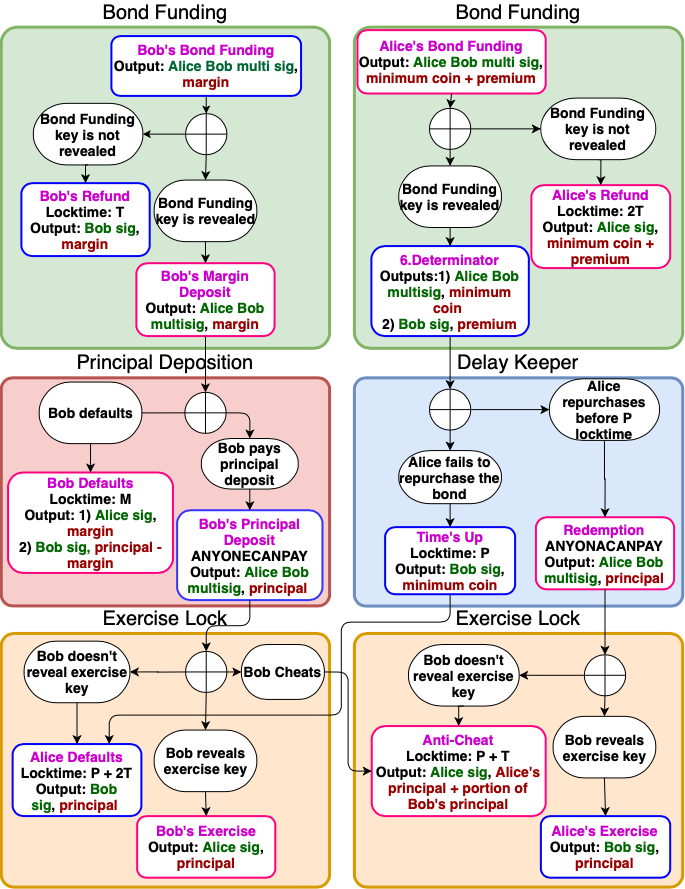
\includegraphics[width=\linewidth]{figures/bond-first.png}
%   \Description{An atomic bonded debt using locktimes}
%   \label{fig:non-collat-bond-no-checkseq}
% \end{figure}
\section{General Overview of Atomic Bonded Debt}
\label{sec:abd}

The idea behind \newfateme{ABCD} is inspired by flash swaps. In a flash swap, the loan is not paid to the borrower unless she pays it back immediately at the same block as borrowed \new{\cite{flashswaps}}. In \abcd this is extended to several blocks i.e. the issuer can \new{repurchase} the bond in more than one block but it contains a secret and the bondholder's signature is required everywhere the capital is being utilized. 

Unsecured bonds or debentures are not backed by some type of collateral. Since this bond is unsecured, the issuer does not have to deposit any margin, unlike the approach used in \new{\cite{liu2018atomic}}. Assume Alice is the issuer and Bob is the purchaser of the bond. She needs to take the capital, exploit it in other contracts, and then \new{repurchase the bond from} Bob with some interest. She also needs Bob to deposit shortly after their contract has been started.

% \subsection{Time Lock based \abcd}
% \label{sub:time-bond}
\newfateme{In this section, we are going to introduce the main challenges for having an atomic bond service. To do so, we designed a general overview of an atomic bond service shown in Fig.}~\ref{fig:non-collat-bond-no-checkseq}. In this , for each transaction, signatures, output amounts, and locktimes are specified. Transactions' border colors show the party who broadcasts the transaction. \newfateme{For now, we assume that all amounts are of the same coin.}
% In this type of bonds, all amounts have to be from the same coin. The cross-chain version of it is discussed later in the section~\ref{sec:abcd}.

\begin{figure}[h]
  \centering
  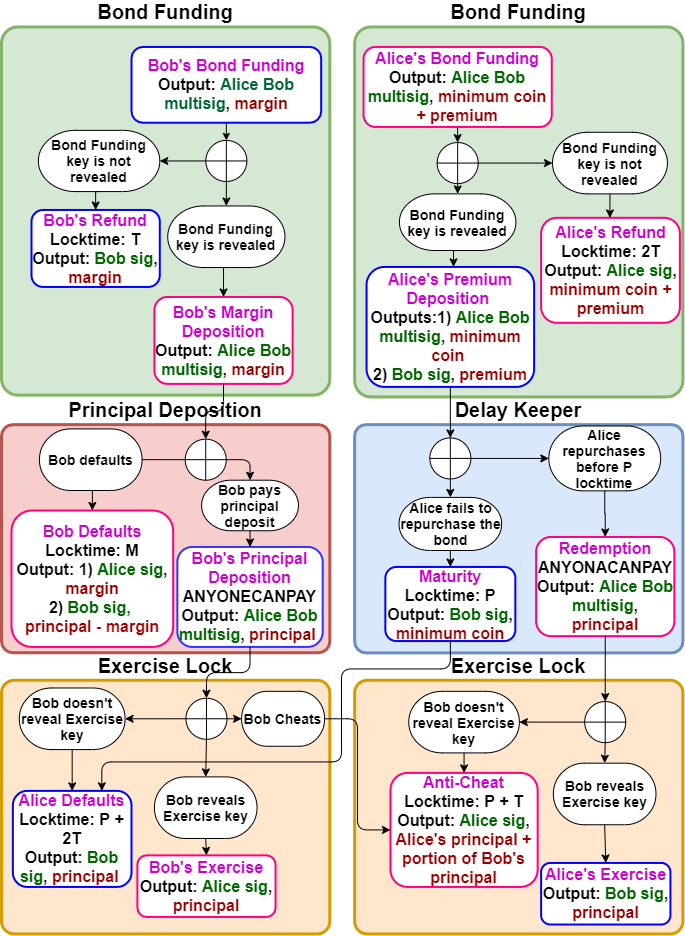
\includegraphics[width=\linewidth]{figures/ABDfateme.png}
  \caption{The general overview of an atomic bond service. Each transaction is shown as a rectangle. On each transaction, signatures, output amount, and locktimes are specified. All outputs are in the same coin. Pink-bordered transactions are broadcast by Alice and blue-bordered ones by Bob. For locktimes, Unix timestamp is used. Upper transactions are broadcast earlier than the lower ones. If there is a line between two transactions, then the source transaction is considered to be an input of the destination transaction.}
  \Description{An atomic bonded debt using locktimes}
  \label{fig:non-collat-bond-no-checkseq}
\end{figure}

Here\newfateme{,} we employ HTLCs to make decisions. If the holder of a secret reveals it before the corresponding timelock deadline, the swap takes place. Otherwise, if she lets the locktime expire, the swap is reverted and all the locked values are given back to their initial owners. The secrets used in \newfateme{this model} are the {\it \Aone} key that the issuer uses to sell and the {\it \keyone} key that the bondholder uses to exercise the bond. In this \newfateme{model}, we use the Unix timestamp as the locktime parameter. We represent the minimum time needed for a mined transaction to be confirmed as $T$. In Bitcoin, it is the time needed to have six subsequent blocks mined which is approximately one hour.

%  Depending on application the bond is being used for, other stages mentioned in the \cite{ourselves} can be appended at the end of the bond structure. The blue box, named as {\it Trust Box} in \cite{ourself} can also be used when the bond is exploited in other contracts such as swaptions \cite{liu2018atomic}, \cite{ourself} i.e. transactions in this boxes may need to be signed by more parties.  Of course in use-cases where additional stages are added, other keys mentioned in \cite{ourself} such as \Atwo key and \Delegation key will be used.

Next\newfateme{,} we explain in detail the process of exercising \newfateme{an atomic bond protocol} which is basically made up of transactions shown in Fig\new{.}~\ref{fig:non-collat-bond-no-checkseq}. First of all, all the transactions are signed and exchanged between the two parties except the bond funding transactions. In this phase, both parties make sure that there is no way the other party cheats on them, since either it is technically impossible or they get punished in case of cheating. This approach is similar to the procedure used by Poon~\etal in the lightening payment channels \new{\cite{poon2016bitcoin}}. After that, by broadcasting each of the transactions in the proper time, the process goes on. The procedure is divided into four different stages. Depending on the application the bond is being used for, other stages can be appended to the procedure and transactions might need to be signed by more parties. However, here we explain the basic structure of the bond itself: 
\begin{itemize}
    \item \textbf{Bond Funding}: 
    The funding transaction for Alice consists of 
    \begin{itemize}
        \item a premium, 
        \item and a very tiny amount for further usage (the minimum acceptable amount of output to be mined by the network miners, for example 546 Satoshis in Bitcoin network at the time of writing).
        % \footnote{In the time we are writing this paper, minimum amount of output in Bitcoin network to be mined by miners is 546 Satoshis}.
    \end{itemize}
    For Bob, the bond funding transaction only contains the margin. Alice has a relatively small amount of time to reveal the \Aone  key to sell the bond. If she issues the bond, the premium goes to Bob and his margin goes to the Bob's margin deposition transaction.
    
    \item \textbf{Principal Deposition}: 
    After selling the bond, each party has to deposit their principal within a specified time interval: Bob $M$ locktime and Alice $P$ ($P > M$). The \emph{\new{Bob's principal} \new{deposition}} and \new{the} \new{\emph{redemption}} transactions have sighash type of anyone-can-pay\footnote{The op-code ANYONECANPAY} since nobody knows all of \newfateme{their} inputs in the first place. Bob can act either ways of:
    \begin{itemize}
        \item If Bob defaults, then Alice takes his margin by broadcasting the \new{\emph{Bob defaults}} transaction. Additionally, she will not fulfill the \newfateme{redemption} transaction. Therefore, Bob can broadcast the \new{\emph{maturity}} transaction, taking the minimum amount of coins which is too small to consider.
        \item If Bob deposits the principal, the bond goes to the \emph{delay keeper} stage.
    \end{itemize}
    The \emph{premium deposition} transaction and the minimum amount of coins are needed so that using this transaction we can force a deadline on Alice depositing her payback by utilizing the locktime on the \new{maturity} transaction. Also, in the case that Alice \new{repurchases} the bond, Bob can not claim that she did not broadcast the \new{redemption} transaction.
    
    \item \textbf{Delay Keeper}: At this stage, Alice has time before a $P$ locktime expires ($P > M$) to fulfill her \new{redemption} transaction. If she does not deposit, Bob will broadcast the \new{maturity} transaction that prevents Alice from fulfilling her \new{redemption} transaction. 
    % Without the presence of the premium deposition transaction, we had no other way to set locktime on the time's up transaction.
    
    \item \textbf{Exercise Lock}: The bond enters this stage when Bob deposits his principal. There are three possible scenarios in here:
    \begin{itemize}
        \item In the last stage, Bob deposited his principal but Alice did not and the \new{maturity} transaction is broadcast. Now Bob does not reveal \keyone key, and using the \new{\emph{Alice defaults}} transaction he takes his principal back.
        
        \item Bob has deposited his principal and Alice has fulfilled her \new{redemption} transaction but Bob avoids revealing the \keyone key. Subsequently, Alice can broadcast the \new{\emph{anti-cheat}} transaction which sends her principal and an amount of punishment from Bob's principal to her. 
        
        \item Both have deposited their principals. Bob reveals \keyone key and they go to the next stage if there is any\footnote{In real-world applications there are usually more stages, since the bond is being used along with other contracts, otherwise it is useless giving ACoins and getting the same ACoins. An example of ABCD implementation along with atomic swap is provided in \cite{abcd-ref}.} and if not, each takes their coins and the procedure ends.
    \end{itemize}

    Note that if Bob delays in broadcasting the \new{maturity} transaction, Alice may broadcast the \new{redemption} and anti-cheat transactions at the very last minute and cheat on Bob.
    
   
\end{itemize}

 \newfateme{The previously presented overview of the atomic bond is well analyzed and seems to be practical. However, there are some problems with its implementation not yet addressed. In every blockchain, signing and spending transactions have a different set of rules,} \new{\eg} \newfateme{in Bitcoin the child transaction has to sign the hash of its parent transaction besides the redeem script. The Bitcoin network considers the inputs of a transaction when calculating its hash. To be able to create a transaction that spends a transaction's output, we need to calculate the parent transaction's hash correctly. Therefore, all of a transaction's inputs have to be determined, before creating its output spender. Hence, the transactions in the exercise lock sections are impossible to be signed at the beginning of the protocol. In the subsequent pages, we will prepare our primitives to overcome this issue.}
